\documentclass[1p]{elsarticle_modified}
%\bibliographystyle{elsarticle-num}

%\usepackage[colorlinks]{hyperref}
%\usepackage{abbrmath_seonhwa} %\Abb, \Ascr, \Acal ,\Abf, \Afrak
\usepackage{amsfonts}
\usepackage{amssymb}
\usepackage{amsmath}
\usepackage{amsthm}
\usepackage{scalefnt}
\usepackage{amsbsy}
\usepackage{kotex}
\usepackage{caption}
\usepackage{subfig}
\usepackage{color}
\usepackage{graphicx}
\usepackage{xcolor} %% white, black, red, green, blue, cyan, magenta, yellow
\usepackage{float}
\usepackage{setspace}
\usepackage{hyperref}

\usepackage{tikz}
\usetikzlibrary{arrows}

\usepackage{multirow}
\usepackage{array} % fixed length table
\usepackage{hhline}

%%%%%%%%%%%%%%%%%%%%%
\makeatletter
\renewcommand*\env@matrix[1][\arraystretch]{%
	\edef\arraystretch{#1}%
	\hskip -\arraycolsep
	\let\@ifnextchar\new@ifnextchar
	\array{*\c@MaxMatrixCols c}}
\makeatother %https://tex.stackexchange.com/questions/14071/how-can-i-increase-the-line-spacing-in-a-matrix
%%%%%%%%%%%%%%%

\usepackage[normalem]{ulem}

\newcommand{\msout}[1]{\ifmmode\text{\sout{\ensuremath{#1}}}\else\sout{#1}\fi}
%SOURCE: \msout is \stkout macro in https://tex.stackexchange.com/questions/20609/strikeout-in-math-mode

\newcommand{\cancel}[1]{
	\ifmmode
	{\color{red}\msout{#1}}
	\else
	{\color{red}\sout{#1}}
	\fi
}

\newcommand{\add}[1]{
	{\color{blue}\uwave{#1}}
}

\newcommand{\replace}[2]{
	\ifmmode
	{\color{red}\msout{#1}}{\color{blue}\uwave{#2}}
	\else
	{\color{red}\sout{#1}}{\color{blue}\uwave{#2}}
	\fi
}

\newcommand{\Sol}{\mathcal{S}} %segment
\newcommand{\D}{D} %diagram
\newcommand{\A}{\mathcal{A}} %arc


%%%%%%%%%%%%%%%%%%%%%%%%%%%%%5 test

\def\sl{\operatorname{\textup{SL}}(2,\Cbb)}
\def\psl{\operatorname{\textup{PSL}}(2,\Cbb)}
\def\quan{\mkern 1mu \triangleright \mkern 1mu}

\theoremstyle{definition}
\newtheorem{thm}{Theorem}[section]
\newtheorem{prop}[thm]{Proposition}
\newtheorem{lem}[thm]{Lemma}
\newtheorem{ques}[thm]{Question}
\newtheorem{cor}[thm]{Corollary}
\newtheorem{defn}[thm]{Definition}
\newtheorem{exam}[thm]{Example}
\newtheorem{rmk}[thm]{Remark}
\newtheorem{alg}[thm]{Algorithm}

\newcommand{\I}{\sqrt{-1}}
\begin{document}

%\begin{frontmatter}
%
%\title{Boundary parabolic representations of knots up to 8 crossings}
%
%%% Group authors per affiliation:
%\author{Yunhi Cho} 
%\address{Department of Mathematics, University of Seoul, Seoul, Korea}
%\ead{yhcho@uos.ac.kr}
%
%
%\author{Seonhwa Kim} %\fnref{s_kim}}
%\address{Center for Geometry and Physics, Institute for Basic Science, Pohang, 37673, Korea}
%\ead{ryeona17@ibs.re.kr}
%
%\author{Hyuk Kim}
%\address{Department of Mathematical Sciences, Seoul National University, Seoul 08826, Korea}
%\ead{hyukkim@snu.ac.kr}
%
%\author{Seokbeom Yoon}
%\address{Department of Mathematical Sciences, Seoul National University, Seoul, 08826,  Korea}
%\ead{sbyoon15@snu.ac.kr}
%
%\begin{abstract}
%We find all boundary parabolic representation of knots up to 8 crossings.
%
%\end{abstract}
%\begin{keyword}
%    \MSC[2010] 57M25 
%\end{keyword}
%
%\end{frontmatter}

%\linenumbers
%\tableofcontents
%
\newcommand\colored[1]{\textcolor{white}{\rule[-0.35ex]{0.8em}{1.4ex}}\kern-0.8em\color{red} #1}%
%\newcommand\colored[1]{\textcolor{white}{ #1}\kern-2.17ex	\textcolor{white}{ #1}\kern-1.81ex	\textcolor{white}{ #1}\kern-2.15ex\color{red}#1	}

{\Large $\underline{12a_{0432}~(K12a_{0432})}$}

\setlength{\tabcolsep}{10pt}
\renewcommand{\arraystretch}{1.6}
\vspace{1cm}\begin{tabular}{m{100pt}>{\centering\arraybackslash}m{274pt}}
\multirow{5}{120pt}{
	\centering
	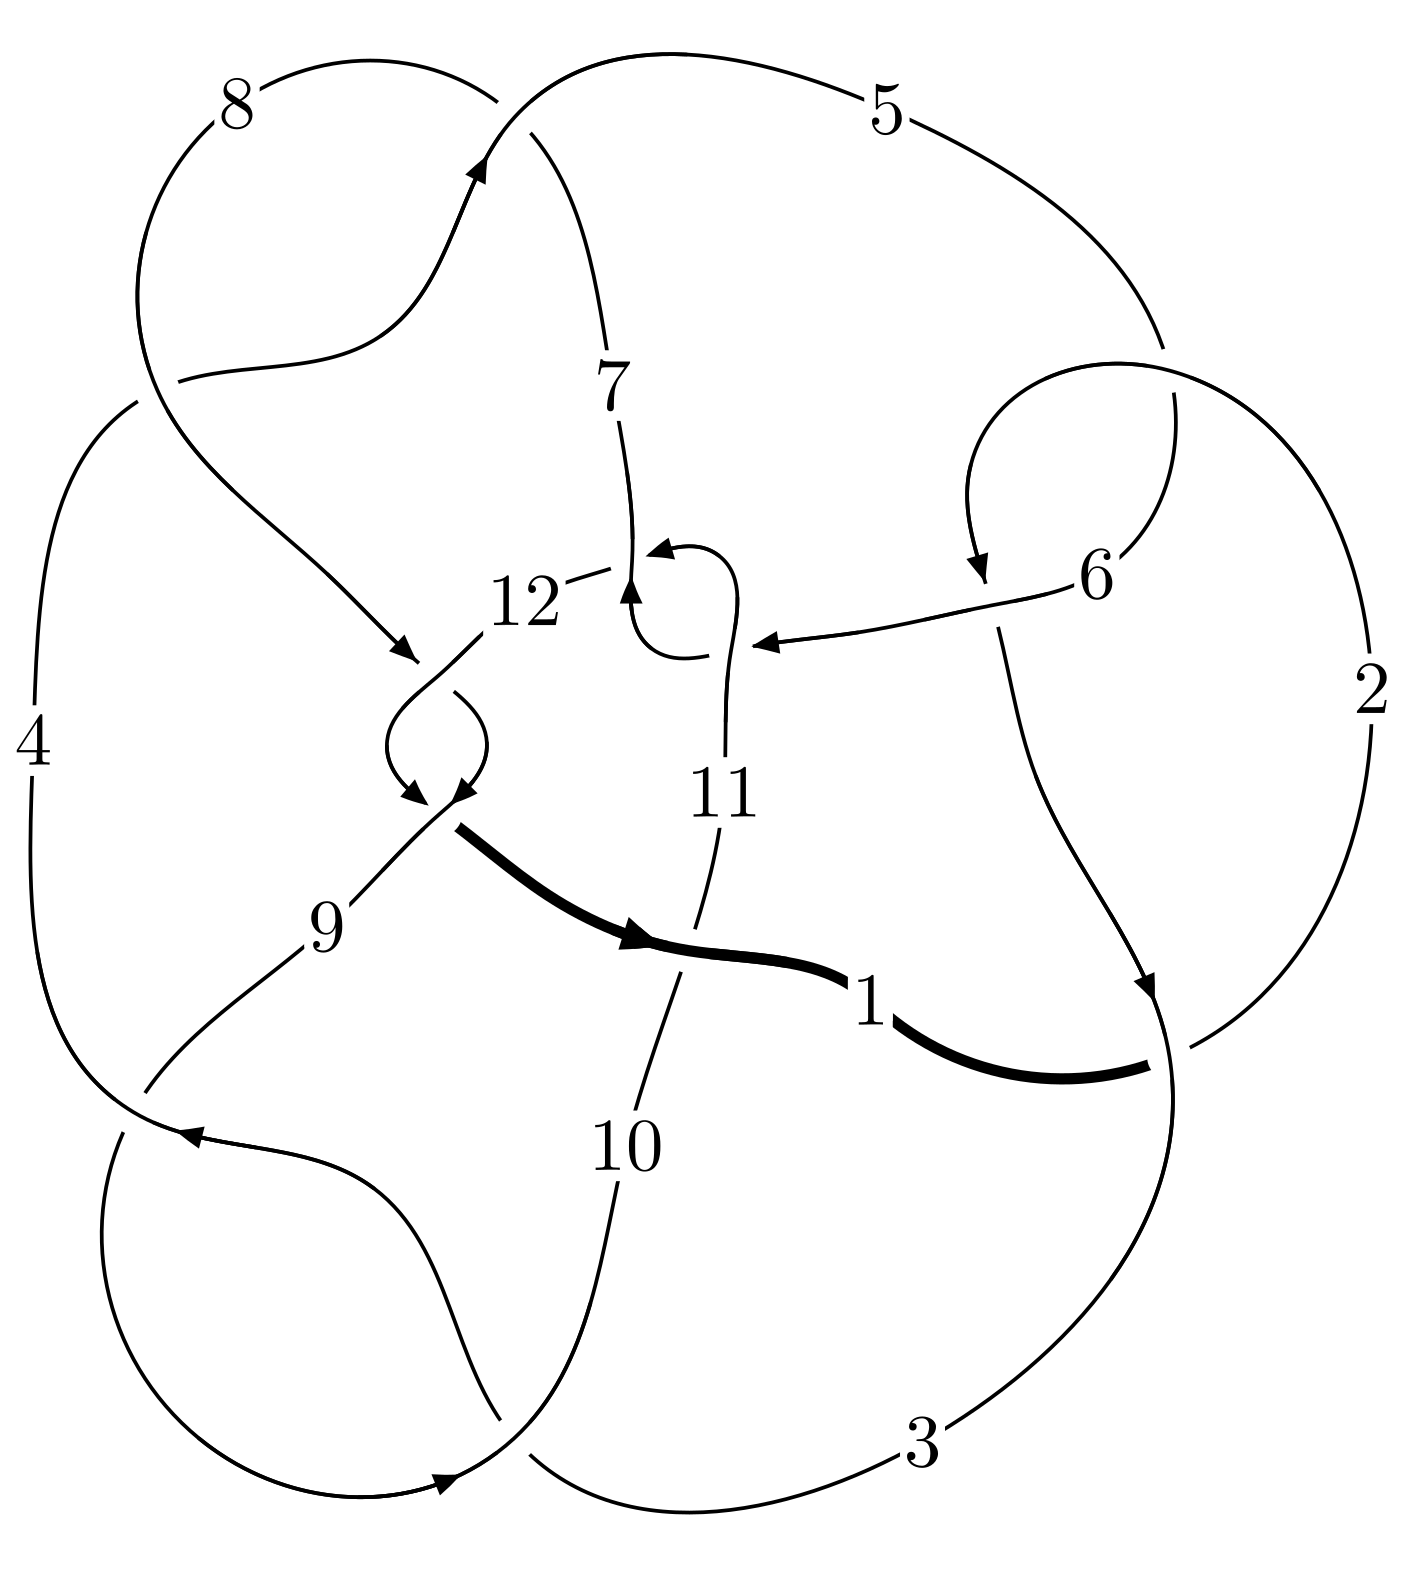
\includegraphics[width=112pt]{../../../GIT/diagram.site/Diagrams/png/1233_12a_0432.png}\\
\ \ \ A knot diagram\footnotemark}&
\allowdisplaybreaks
\textbf{Linearized knot diagam} \\
\cline{2-2}
 &
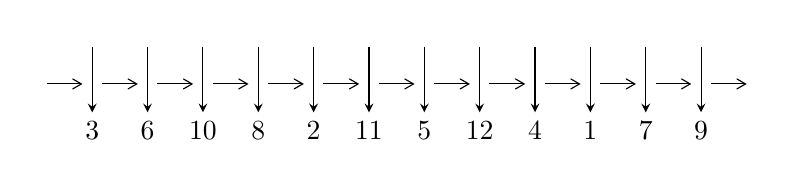
\begin{tikzpicture}[x=20pt, y=17pt]
	% nodes
	\node (C0) at (0, 0) {};
	\node (C1) at (1, 0) {};
	\node (C1U) at (1, +1) {};
	\node (C1D) at (1, -1) {3};

	\node (C2) at (2, 0) {};
	\node (C2U) at (2, +1) {};
	\node (C2D) at (2, -1) {6};

	\node (C3) at (3, 0) {};
	\node (C3U) at (3, +1) {};
	\node (C3D) at (3, -1) {10};

	\node (C4) at (4, 0) {};
	\node (C4U) at (4, +1) {};
	\node (C4D) at (4, -1) {8};

	\node (C5) at (5, 0) {};
	\node (C5U) at (5, +1) {};
	\node (C5D) at (5, -1) {2};

	\node (C6) at (6, 0) {};
	\node (C6U) at (6, +1) {};
	\node (C6D) at (6, -1) {11};

	\node (C7) at (7, 0) {};
	\node (C7U) at (7, +1) {};
	\node (C7D) at (7, -1) {5};

	\node (C8) at (8, 0) {};
	\node (C8U) at (8, +1) {};
	\node (C8D) at (8, -1) {12};

	\node (C9) at (9, 0) {};
	\node (C9U) at (9, +1) {};
	\node (C9D) at (9, -1) {4};

	\node (C10) at (10, 0) {};
	\node (C10U) at (10, +1) {};
	\node (C10D) at (10, -1) {1};

	\node (C11) at (11, 0) {};
	\node (C11U) at (11, +1) {};
	\node (C11D) at (11, -1) {7};

	\node (C12) at (12, 0) {};
	\node (C12U) at (12, +1) {};
	\node (C12D) at (12, -1) {9};
	\node (C13) at (13, 0) {};

	% arrows
	\draw[->,>={angle 60}]
	(C0) edge (C1) (C1) edge (C2) (C2) edge (C3) (C3) edge (C4) (C4) edge (C5) (C5) edge (C6) (C6) edge (C7) (C7) edge (C8) (C8) edge (C9) (C9) edge (C10) (C10) edge (C11) (C11) edge (C12) (C12) edge (C13) ;	\draw[->,>=stealth]
	(C1U) edge (C1D) (C2U) edge (C2D) (C3U) edge (C3D) (C4U) edge (C4D) (C5U) edge (C5D) (C6U) edge (C6D) (C7U) edge (C7D) (C8U) edge (C8D) (C9U) edge (C9D) (C10U) edge (C10D) (C11U) edge (C11D) (C12U) edge (C12D) ;
	\end{tikzpicture} \\
\hhline{~~} \\& 
\textbf{Solving Sequence} \\ \cline{2-2} 
 &
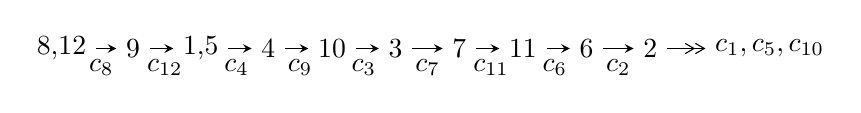
\begin{tikzpicture}[x=23pt, y=7pt]
	% node
	\node (A0) at (-1/8, 0) {8,12};
	\node (A1) at (1, 0) {9};
	\node (A2) at (33/16, 0) {1,5};
	\node (A3) at (25/8, 0) {4};
	\node (A4) at (33/8, 0) {10};
	\node (A5) at (41/8, 0) {3};
	\node (A6) at (49/8, 0) {7};
	\node (A7) at (57/8, 0) {11};
	\node (A8) at (65/8, 0) {6};
	\node (A9) at (73/8, 0) {2};
	\node (C1) at (1/2, -1) {$c_{8}$};
	\node (C2) at (3/2, -1) {$c_{12}$};
	\node (C3) at (21/8, -1) {$c_{4}$};
	\node (C4) at (29/8, -1) {$c_{9}$};
	\node (C5) at (37/8, -1) {$c_{3}$};
	\node (C6) at (45/8, -1) {$c_{7}$};
	\node (C7) at (53/8, -1) {$c_{11}$};
	\node (C8) at (61/8, -1) {$c_{6}$};
	\node (C9) at (69/8, -1) {$c_{2}$};
	\node (A10) at (11, 0) {$c_{1},c_{5},c_{10}$};

	% edge
	\draw[->,>=stealth]	
	(A0) edge (A1) (A1) edge (A2) (A2) edge (A3) (A3) edge (A4) (A4) edge (A5) (A5) edge (A6) (A6) edge (A7) (A7) edge (A8) (A8) edge (A9) ;
	\draw[->>,>={angle 60}]	
	(A9) edge (A10);
\end{tikzpicture} \\ 

\end{tabular} \\

\footnotetext{
The image of knot diagram is generated by the software ``\textbf{Draw programme}" developed by Andrew Bartholomew(\url{http://www.layer8.co.uk/maths/draw/index.htm\#Running-draw}), where we modified some parts for our purpose(\url{https://github.com/CATsTAILs/LinksPainter}).
}\phantom \\ \newline 
\centering \textbf{Ideals for irreducible components\footnotemark of $X_{\text{par}}$} 
 
\begin{align*}
I^u_{1}&=\langle 
8.17956\times10^{513} u^{126}+6.56820\times10^{513} u^{125}+\cdots+6.50124\times10^{510} b+9.89260\times10^{513},\\
\phantom{I^u_{1}}&\phantom{= \langle  }-2.16012\times10^{513} u^{126}-2.23997\times10^{513} u^{125}+\cdots+6.50124\times10^{510} a-8.59599\times10^{512},\\
\phantom{I^u_{1}}&\phantom{= \langle  }u^{127}-39 u^{125}+\cdots+26 u-1\rangle \\
I^u_{2}&=\langle 
-1683522 u^{21}-10851287 u^{20}+\cdots+135991 b+8481275,\\
\phantom{I^u_{2}}&\phantom{= \langle  }191582 u^{21}+1200977 u^{20}+\cdots+407973 a+2348438,\;u^{22}+7 u^{21}+\cdots-11 u-3\rangle \\
\\
\end{align*}
\raggedright * 2 irreducible components of $\dim_{\mathbb{C}}=0$, with total 149 representations.\\
\footnotetext{All coefficients of polynomials are rational numbers. But the coefficients are sometimes approximated in decimal forms when there is not enough margin.}
\newpage
\renewcommand{\arraystretch}{1}
\centering \section*{I. $I^u_{1}= \langle 8.18\times10^{513} u^{126}+6.57\times10^{513} u^{125}+\cdots+6.50\times10^{510} b+9.89\times10^{513},\;-2.16\times10^{513} u^{126}-2.24\times10^{513} u^{125}+\cdots+6.50\times10^{510} a-8.60\times10^{512},\;u^{127}-39 u^{125}+\cdots+26 u-1 \rangle$}
\flushleft \textbf{(i) Arc colorings}\\
\begin{tabular}{m{7pt} m{180pt} m{7pt} m{180pt} }
\flushright $a_{8}=$&$\begin{pmatrix}1\\0\end{pmatrix}$ \\
\flushright $a_{12}=$&$\begin{pmatrix}0\\u\end{pmatrix}$ \\
\flushright $a_{9}=$&$\begin{pmatrix}1\\u^2\end{pmatrix}$ \\
\flushright $a_{1}=$&$\begin{pmatrix}- u\\- u^3+u\end{pmatrix}$ \\
\flushright $a_{5}=$&$\begin{pmatrix}332.262 u^{126}+344.545 u^{125}+\cdots-4418.94 u+132.221\\-1258.15 u^{126}-1010.30 u^{125}+\cdots+37831.1 u-1521.65\end{pmatrix}$ \\
\flushright $a_{4}=$&$\begin{pmatrix}-925.891 u^{126}-665.754 u^{125}+\cdots+33412.1 u-1389.43\\-1258.15 u^{126}-1010.30 u^{125}+\cdots+37831.1 u-1521.65\end{pmatrix}$ \\
\flushright $a_{10}=$&$\begin{pmatrix}124.346 u^{126}-35.5978 u^{125}+\cdots-11588.4 u+504.585\\35.6942 u^{126}-15.6952 u^{125}+\cdots-3727.56 u+160.148\end{pmatrix}$ \\
\flushright $a_{3}=$&$\begin{pmatrix}-102.852 u^{126}-177.716 u^{125}+\cdots-1620.58 u+63.8561\\1184.64 u^{126}+900.526 u^{125}+\cdots-39219.1 u+1594.14\end{pmatrix}$ \\
\flushright $a_{7}=$&$\begin{pmatrix}-54.1645 u^{126}-4.38579 u^{125}+\cdots+3562.79 u-159.539\\210.170 u^{126}+240.717 u^{125}+\cdots-2261.06 u+76.1834\end{pmatrix}$ \\
\flushright $a_{11}=$&$\begin{pmatrix}154.927 u^{126}+24.7007 u^{125}+\cdots-10450.6 u+451.072\\70.7956 u^{126}-14.9643 u^{125}+\cdots-6402.55 u+273.959\end{pmatrix}$ \\
\flushright $a_{6}=$&$\begin{pmatrix}185.571 u^{126}+68.9838 u^{125}+\cdots-11041.8 u+462.863\\433.621 u^{126}+356.001 u^{125}+\cdots-12831.4 u+516.286\end{pmatrix}$ \\
\flushright $a_{2}=$&$\begin{pmatrix}-73.6548 u^{126}-61.8141 u^{125}+\cdots+3792.30 u-186.708\\222.809 u^{126}+191.525 u^{125}+\cdots-6309.64 u+253.297\end{pmatrix}$\\&\end{tabular}
\flushleft \textbf{(ii) Obstruction class $= -1$}\\~\\
\flushleft \textbf{(iii) Cusp Shapes $= -1954.67 u^{126}-1603.54 u^{125}+\cdots+57833.4 u-2355.39$}\\~\\
\newpage\renewcommand{\arraystretch}{1}
\flushleft \textbf{(iv) u-Polynomials at the component}\newline \\
\begin{tabular}{m{50pt}|m{274pt}}
Crossings & \hspace{64pt}u-Polynomials at each crossing \\
\hline $$\begin{aligned}c_{1}\end{aligned}$$&$\begin{aligned}
&u^{127}+51 u^{126}+\cdots+64748 u+961
\end{aligned}$\\
\hline $$\begin{aligned}c_{2},c_{5}\end{aligned}$$&$\begin{aligned}
&u^{127}+3 u^{126}+\cdots-322 u+31
\end{aligned}$\\
\hline $$\begin{aligned}c_{3},c_{9}\end{aligned}$$&$\begin{aligned}
&u^{127}+5 u^{126}+\cdots+33188 u+3019
\end{aligned}$\\
\hline $$\begin{aligned}c_{4},c_{7}\end{aligned}$$&$\begin{aligned}
&u^{127}-4 u^{126}+\cdots-8 u+1
\end{aligned}$\\
\hline $$\begin{aligned}c_{6},c_{11}\end{aligned}$$&$\begin{aligned}
&u^{127}-2 u^{126}+\cdots+2124 u+3559
\end{aligned}$\\
\hline $$\begin{aligned}c_{8},c_{12}\end{aligned}$$&$\begin{aligned}
&u^{127}-39 u^{125}+\cdots+26 u+1
\end{aligned}$\\
\hline $$\begin{aligned}c_{10}\end{aligned}$$&$\begin{aligned}
&u^{127}-2 u^{126}+\cdots+12444 u+1273
\end{aligned}$\\
\hline
\end{tabular}\\~\\
\newpage\renewcommand{\arraystretch}{1}
\flushleft \textbf{(v) Riley Polynomials at the component}\newline \\
\begin{tabular}{m{50pt}|m{274pt}}
Crossings & \hspace{64pt}Riley Polynomials at each crossing \\
\hline $$\begin{aligned}c_{1}\end{aligned}$$&$\begin{aligned}
&y^{127}+61 y^{126}+\cdots+252764728 y-923521
\end{aligned}$\\
\hline $$\begin{aligned}c_{2},c_{5}\end{aligned}$$&$\begin{aligned}
&y^{127}-51 y^{126}+\cdots+64748 y-961
\end{aligned}$\\
\hline $$\begin{aligned}c_{3},c_{9}\end{aligned}$$&$\begin{aligned}
&y^{127}+87 y^{126}+\cdots-136207782 y-9114361
\end{aligned}$\\
\hline $$\begin{aligned}c_{4},c_{7}\end{aligned}$$&$\begin{aligned}
&y^{127}+80 y^{126}+\cdots+104 y-1
\end{aligned}$\\
\hline $$\begin{aligned}c_{6},c_{11}\end{aligned}$$&$\begin{aligned}
&y^{127}-74 y^{126}+\cdots+113971980 y-12666481
\end{aligned}$\\
\hline $$\begin{aligned}c_{8},c_{12}\end{aligned}$$&$\begin{aligned}
&y^{127}-78 y^{126}+\cdots+108 y-1
\end{aligned}$\\
\hline $$\begin{aligned}c_{10}\end{aligned}$$&$\begin{aligned}
&y^{127}+10 y^{126}+\cdots-40468346 y-1620529
\end{aligned}$\\
\hline
\end{tabular}\\~\\
\newpage\flushleft \textbf{(vi) Complex Volumes and Cusp Shapes}
$$\begin{array}{c|c|c}  
\text{Solutions to }I^u_{1}& \I (\text{vol} + \sqrt{-1}CS) & \text{Cusp shape}\\
 \hline 
\begin{aligned}
u &= \phantom{-}0.924683 + 0.369839 I \\
a &= \phantom{-}0.608340 - 1.273530 I \\
b &= \phantom{-}0.388767 + 0.488604 I\end{aligned}
 & -2.30026 - 2.96450 I & \phantom{-0.000000 } 0 \\ \hline\begin{aligned}
u &= \phantom{-}0.924683 - 0.369839 I \\
a &= \phantom{-}0.608340 + 1.273530 I \\
b &= \phantom{-}0.388767 - 0.488604 I\end{aligned}
 & -2.30026 + 2.96450 I & \phantom{-0.000000 } 0 \\ \hline\begin{aligned}
u &= \phantom{-}1.001120 + 0.147493 I \\
a &= -3.19117 + 0.15377 I \\
b &= -0.089038 - 0.925983 I\end{aligned}
 & -0.14172 - 2.38640 I & \phantom{-0.000000 } 0 \\ \hline\begin{aligned}
u &= \phantom{-}1.001120 - 0.147493 I \\
a &= -3.19117 - 0.15377 I \\
b &= -0.089038 + 0.925983 I\end{aligned}
 & -0.14172 + 2.38640 I & \phantom{-0.000000 } 0 \\ \hline\begin{aligned}
u &= \phantom{-}0.978649 + 0.131591 I \\
a &= \phantom{-}0.112195 - 1.062580 I \\
b &= \phantom{-}0.143483 + 0.046794 I\end{aligned}
 & -1.71435 + 2.00781 I & \phantom{-0.000000 } 0 \\ \hline\begin{aligned}
u &= \phantom{-}0.978649 - 0.131591 I \\
a &= \phantom{-}0.112195 + 1.062580 I \\
b &= \phantom{-}0.143483 - 0.046794 I\end{aligned}
 & -1.71435 - 2.00781 I & \phantom{-0.000000 } 0 \\ \hline\begin{aligned}
u &= \phantom{-}0.782053 + 0.653717 I \\
a &= -0.55451 + 1.69182 I \\
b &= -0.550760 - 0.827776 I\end{aligned}
 & -2.79611 - 0.76104 I & \phantom{-0.000000 } 0 \\ \hline\begin{aligned}
u &= \phantom{-}0.782053 - 0.653717 I \\
a &= -0.55451 - 1.69182 I \\
b &= -0.550760 + 0.827776 I\end{aligned}
 & -2.79611 + 0.76104 I & \phantom{-0.000000 } 0 \\ \hline\begin{aligned}
u &= -0.174076 + 1.005220 I \\
a &= \phantom{-}0.05242 - 1.45375 I \\
b &= \phantom{-}0.127324 + 1.393990 I\end{aligned}
 & \phantom{-}8.45647 - 6.32148 I & \phantom{-0.000000 } 0 \\ \hline\begin{aligned}
u &= -0.174076 - 1.005220 I \\
a &= \phantom{-}0.05242 + 1.45375 I \\
b &= \phantom{-}0.127324 - 1.393990 I\end{aligned}
 & \phantom{-}8.45647 + 6.32148 I & \phantom{-0.000000 } 0\\
 \hline 
 \end{array}$$\newpage$$\begin{array}{c|c|c}  
\text{Solutions to }I^u_{1}& \I (\text{vol} + \sqrt{-1}CS) & \text{Cusp shape}\\
 \hline 
\begin{aligned}
u &= \phantom{-}1.058630 + 0.164072 I \\
a &= \phantom{-}2.33472 + 0.80946 I \\
b &= \phantom{-}0.059832 + 0.858484 I\end{aligned}
 & -0.38624 + 1.70611 I & \phantom{-0.000000 } 0 \\ \hline\begin{aligned}
u &= \phantom{-}1.058630 - 0.164072 I \\
a &= \phantom{-}2.33472 - 0.80946 I \\
b &= \phantom{-}0.059832 - 0.858484 I\end{aligned}
 & -0.38624 - 1.70611 I & \phantom{-0.000000 } 0 \\ \hline\begin{aligned}
u &= -0.836922 + 0.378466 I \\
a &= \phantom{-}0.674692 + 0.298321 I \\
b &= \phantom{-}0.795291 + 0.260018 I\end{aligned}
 & -2.03359 + 1.57618 I & \phantom{-0.000000 } 0 \\ \hline\begin{aligned}
u &= -0.836922 - 0.378466 I \\
a &= \phantom{-}0.674692 - 0.298321 I \\
b &= \phantom{-}0.795291 - 0.260018 I\end{aligned}
 & -2.03359 - 1.57618 I & \phantom{-0.000000 } 0 \\ \hline\begin{aligned}
u &= \phantom{-}1.005480 + 0.400774 I \\
a &= -0.980953 + 0.573737 I \\
b &= -0.087151 - 0.903960 I\end{aligned}
 & -0.298985 - 0.775562 I & \phantom{-0.000000 } 0 \\ \hline\begin{aligned}
u &= \phantom{-}1.005480 - 0.400774 I \\
a &= -0.980953 - 0.573737 I \\
b &= -0.087151 + 0.903960 I\end{aligned}
 & -0.298985 + 0.775562 I & \phantom{-0.000000 } 0 \\ \hline\begin{aligned}
u &= -0.727229 + 0.555930 I \\
a &= -1.297510 - 0.284976 I \\
b &= -0.200909 - 0.061435 I\end{aligned}
 & \phantom{-}2.78595 + 3.48689 I & \phantom{-0.000000 } 0 \\ \hline\begin{aligned}
u &= -0.727229 - 0.555930 I \\
a &= -1.297510 + 0.284976 I \\
b &= -0.200909 + 0.061435 I\end{aligned}
 & \phantom{-}2.78595 - 3.48689 I & \phantom{-0.000000 } 0 \\ \hline\begin{aligned}
u &= -0.225415 + 1.071830 I \\
a &= -0.094820 + 1.372120 I \\
b &= -0.057743 - 1.348270 I\end{aligned}
 & \phantom{-}9.41775 - 0.48167 I & \phantom{-0.000000 } 0 \\ \hline\begin{aligned}
u &= -0.225415 - 1.071830 I \\
a &= -0.094820 - 1.372120 I \\
b &= -0.057743 + 1.348270 I\end{aligned}
 & \phantom{-}9.41775 + 0.48167 I & \phantom{-0.000000 } 0\\
 \hline 
 \end{array}$$\newpage$$\begin{array}{c|c|c}  
\text{Solutions to }I^u_{1}& \I (\text{vol} + \sqrt{-1}CS) & \text{Cusp shape}\\
 \hline 
\begin{aligned}
u &= \phantom{-}0.884516 + 0.055608 I \\
a &= -1.73570 + 3.59443 I \\
b &= -0.084782 - 1.096170 I\end{aligned}
 & \phantom{-}0.31178 + 1.84948 I & \phantom{-0.000000 } 0 \\ \hline\begin{aligned}
u &= \phantom{-}0.884516 - 0.055608 I \\
a &= -1.73570 - 3.59443 I \\
b &= -0.084782 + 1.096170 I\end{aligned}
 & \phantom{-}0.31178 - 1.84948 I & \phantom{-0.000000 } 0 \\ \hline\begin{aligned}
u &= \phantom{-}1.009010 + 0.472200 I \\
a &= -0.828558 + 0.588752 I \\
b &= \phantom{-}0.021031 - 0.929926 I\end{aligned}
 & -0.275081 - 0.781566 I & \phantom{-0.000000 } 0 \\ \hline\begin{aligned}
u &= \phantom{-}1.009010 - 0.472200 I \\
a &= -0.828558 - 0.588752 I \\
b &= \phantom{-}0.021031 + 0.929926 I\end{aligned}
 & -0.275081 + 0.781566 I & \phantom{-0.000000 } 0 \\ \hline\begin{aligned}
u &= -0.616167 + 0.577419 I \\
a &= \phantom{-}1.85521 + 0.68990 I \\
b &= -0.0724564 - 0.0703583 I\end{aligned}
 & \phantom{-}0.69570 + 8.80811 I & \phantom{-0.000000 } 0 \\ \hline\begin{aligned}
u &= -0.616167 - 0.577419 I \\
a &= \phantom{-}1.85521 - 0.68990 I \\
b &= -0.0724564 + 0.0703583 I\end{aligned}
 & \phantom{-}0.69570 - 8.80811 I & \phantom{-0.000000 } 0 \\ \hline\begin{aligned}
u &= -1.015590 + 0.560681 I \\
a &= \phantom{-}0.720345 + 0.732910 I \\
b &= \phantom{-}0.931075 - 0.511817 I\end{aligned}
 & \phantom{-}0.42465 + 8.09284 I & \phantom{-0.000000 } 0 \\ \hline\begin{aligned}
u &= -1.015590 - 0.560681 I \\
a &= \phantom{-}0.720345 - 0.732910 I \\
b &= \phantom{-}0.931075 + 0.511817 I\end{aligned}
 & \phantom{-}0.42465 - 8.09284 I & \phantom{-0.000000 } 0 \\ \hline\begin{aligned}
u &= \phantom{-}1.154410 + 0.236419 I \\
a &= \phantom{-}0.813409 + 0.475466 I \\
b &= \phantom{-}0.276136 + 0.626016 I\end{aligned}
 & -1.27774 - 2.53272 I & \phantom{-0.000000 } 0 \\ \hline\begin{aligned}
u &= \phantom{-}1.154410 - 0.236419 I \\
a &= \phantom{-}0.813409 - 0.475466 I \\
b &= \phantom{-}0.276136 - 0.626016 I\end{aligned}
 & -1.27774 + 2.53272 I & \phantom{-0.000000 } 0\\
 \hline 
 \end{array}$$\newpage$$\begin{array}{c|c|c}  
\text{Solutions to }I^u_{1}& \I (\text{vol} + \sqrt{-1}CS) & \text{Cusp shape}\\
 \hline 
\begin{aligned}
u &= -1.050520 + 0.536489 I \\
a &= \phantom{-}0.784616 + 0.920323 I \\
b &= \phantom{-}1.00707 - 1.29629 I\end{aligned}
 & \phantom{-}2.37250 + 3.37648 I & \phantom{-0.000000 } 0 \\ \hline\begin{aligned}
u &= -1.050520 - 0.536489 I \\
a &= \phantom{-}0.784616 - 0.920323 I \\
b &= \phantom{-}1.00707 + 1.29629 I\end{aligned}
 & \phantom{-}2.37250 - 3.37648 I & \phantom{-0.000000 } 0 \\ \hline\begin{aligned}
u &= -1.052630 + 0.553384 I \\
a &= -0.767236 - 0.924602 I \\
b &= -1.10195 + 1.21661 I\end{aligned}
 & \phantom{-}2.29330 + 7.94168 I & \phantom{-0.000000 } 0 \\ \hline\begin{aligned}
u &= -1.052630 - 0.553384 I \\
a &= -0.767236 + 0.924602 I \\
b &= -1.10195 - 1.21661 I\end{aligned}
 & \phantom{-}2.29330 - 7.94168 I & \phantom{-0.000000 } 0 \\ \hline\begin{aligned}
u &= -0.452818 + 0.667940 I \\
a &= \phantom{-}0.824452 + 0.566550 I \\
b &= -0.53812 - 1.42737 I\end{aligned}
 & \phantom{-}4.04606 - 3.19347 I & \phantom{-0.000000 } 0 \\ \hline\begin{aligned}
u &= -0.452818 - 0.667940 I \\
a &= \phantom{-}0.824452 - 0.566550 I \\
b &= -0.53812 + 1.42737 I\end{aligned}
 & \phantom{-}4.04606 + 3.19347 I & \phantom{-0.000000 } 0 \\ \hline\begin{aligned}
u &= -0.445440 + 0.666343 I \\
a &= \phantom{-}0.434019 + 0.485862 I \\
b &= -0.532311 - 1.119660 I\end{aligned}
 & \phantom{-}3.15024 + 0.50709 I & \phantom{-0.000000 } 0 \\ \hline\begin{aligned}
u &= -0.445440 - 0.666343 I \\
a &= \phantom{-}0.434019 - 0.485862 I \\
b &= -0.532311 + 1.119660 I\end{aligned}
 & \phantom{-}3.15024 - 0.50709 I & \phantom{-0.000000 } 0 \\ \hline\begin{aligned}
u &= -0.601574 + 0.523680 I \\
a &= -0.446446 + 0.178316 I \\
b &= -0.412904 - 0.638276 I\end{aligned}
 & \phantom{-}3.19727 + 0.99504 I & \phantom{-0.000000 } 0 \\ \hline\begin{aligned}
u &= -0.601574 - 0.523680 I \\
a &= -0.446446 - 0.178316 I \\
b &= -0.412904 + 0.638276 I\end{aligned}
 & \phantom{-}3.19727 - 0.99504 I & \phantom{-0.000000 } 0\\
 \hline 
 \end{array}$$\newpage$$\begin{array}{c|c|c}  
\text{Solutions to }I^u_{1}& \I (\text{vol} + \sqrt{-1}CS) & \text{Cusp shape}\\
 \hline 
\begin{aligned}
u &= -1.060950 + 0.566207 I \\
a &= -0.730209 - 0.864846 I \\
b &= -1.069190 + 0.900490 I\end{aligned}
 & \phantom{-}1.35731 + 4.29706 I & \phantom{-0.000000 } 0 \\ \hline\begin{aligned}
u &= -1.060950 - 0.566207 I \\
a &= -0.730209 + 0.864846 I \\
b &= -1.069190 - 0.900490 I\end{aligned}
 & \phantom{-}1.35731 - 4.29706 I & \phantom{-0.000000 } 0 \\ \hline\begin{aligned}
u &= -0.459921 + 0.648792 I \\
a &= -0.884835 - 0.659165 I \\
b &= \phantom{-}0.43189 + 1.47336 I\end{aligned}
 & \phantom{-}4.10482 + 1.26411 I & \phantom{-0.000000 } 0 \\ \hline\begin{aligned}
u &= -0.459921 - 0.648792 I \\
a &= -0.884835 + 0.659165 I \\
b &= \phantom{-}0.43189 - 1.47336 I\end{aligned}
 & \phantom{-}4.10482 - 1.26411 I & \phantom{-0.000000 } 0 \\ \hline\begin{aligned}
u &= \phantom{-}1.141480 + 0.404863 I \\
a &= \phantom{-}0.0260910 + 0.0015194 I \\
b &= -1.53189 + 0.29731 I\end{aligned}
 & -2.64906 - 11.55230 I & \phantom{-0.000000 } 0 \\ \hline\begin{aligned}
u &= \phantom{-}1.141480 - 0.404863 I \\
a &= \phantom{-}0.0260910 - 0.0015194 I \\
b &= -1.53189 - 0.29731 I\end{aligned}
 & -2.64906 + 11.55230 I & \phantom{-0.000000 } 0 \\ \hline\begin{aligned}
u &= \phantom{-}1.159150 + 0.383790 I \\
a &= \phantom{-}0.0210091 + 0.0368586 I \\
b &= \phantom{-}1.44124 - 0.15234 I\end{aligned}
 & -1.07882 - 5.87309 I & \phantom{-0.000000 } 0 \\ \hline\begin{aligned}
u &= \phantom{-}1.159150 - 0.383790 I \\
a &= \phantom{-}0.0210091 - 0.0368586 I \\
b &= \phantom{-}1.44124 + 0.15234 I\end{aligned}
 & -1.07882 + 5.87309 I & \phantom{-0.000000 } 0 \\ \hline\begin{aligned}
u &= \phantom{-}0.773781 + 0.006379 I \\
a &= \phantom{-}0.096914 + 0.879200 I \\
b &= \phantom{-}0.15875 - 2.30172 I\end{aligned}
 & \phantom{-}6.59700 + 2.90052 I & \phantom{-0.000000 } 0 \\ \hline\begin{aligned}
u &= \phantom{-}0.773781 - 0.006379 I \\
a &= \phantom{-}0.096914 - 0.879200 I \\
b &= \phantom{-}0.15875 + 2.30172 I\end{aligned}
 & \phantom{-}6.59700 - 2.90052 I & \phantom{-0.000000 } 0\\
 \hline 
 \end{array}$$\newpage$$\begin{array}{c|c|c}  
\text{Solutions to }I^u_{1}& \I (\text{vol} + \sqrt{-1}CS) & \text{Cusp shape}\\
 \hline 
\begin{aligned}
u &= \phantom{-}0.737225 + 0.083244 I \\
a &= \phantom{-}1.12451 - 1.75733 I \\
b &= \phantom{-}0.397770 + 1.232700 I\end{aligned}
 & \phantom{-}1.43975 - 1.67693 I & \phantom{-0.000000 } 0 \\ \hline\begin{aligned}
u &= \phantom{-}0.737225 - 0.083244 I \\
a &= \phantom{-}1.12451 + 1.75733 I \\
b &= \phantom{-}0.397770 - 1.232700 I\end{aligned}
 & \phantom{-}1.43975 + 1.67693 I & \phantom{-0.000000 } 0 \\ \hline\begin{aligned}
u &= -0.318561 + 0.665718 I \\
a &= -0.653109 - 1.207280 I \\
b &= \phantom{-}0.274464 + 1.243040 I\end{aligned}
 & \phantom{-}2.85662 - 2.16898 I & \phantom{-0.000000 } 0 \\ \hline\begin{aligned}
u &= -0.318561 - 0.665718 I \\
a &= -0.653109 + 1.207280 I \\
b &= \phantom{-}0.274464 - 1.243040 I\end{aligned}
 & \phantom{-}2.85662 + 2.16898 I & \phantom{-0.000000 } 0 \\ \hline\begin{aligned}
u &= -1.269100 + 0.104073 I \\
a &= \phantom{-}0.0726301 + 0.1055050 I \\
b &= \phantom{-}1.085320 + 0.179204 I\end{aligned}
 & -5.27482 + 1.33689 I & \phantom{-0.000000 } 0 \\ \hline\begin{aligned}
u &= -1.269100 - 0.104073 I \\
a &= \phantom{-}0.0726301 - 0.1055050 I \\
b &= \phantom{-}1.085320 - 0.179204 I\end{aligned}
 & -5.27482 - 1.33689 I & \phantom{-0.000000 } 0 \\ \hline\begin{aligned}
u &= \phantom{-}0.097674 + 1.269920 I \\
a &= \phantom{-}0.31176 + 1.64860 I \\
b &= -0.342279 - 0.755360 I\end{aligned}
 & -3.11716 - 0.32407 I & \phantom{-0.000000 } 0 \\ \hline\begin{aligned}
u &= \phantom{-}0.097674 - 1.269920 I \\
a &= \phantom{-}0.31176 - 1.64860 I \\
b &= -0.342279 + 0.755360 I\end{aligned}
 & -3.11716 + 0.32407 I & \phantom{-0.000000 } 0 \\ \hline\begin{aligned}
u &= -1.197100 + 0.437234 I \\
a &= \phantom{-}0.75198 + 1.29733 I \\
b &= \phantom{-}0.597393 - 1.278020 I\end{aligned}
 & -1.84583 + 7.27986 I & \phantom{-0.000000 } 0 \\ \hline\begin{aligned}
u &= -1.197100 - 0.437234 I \\
a &= \phantom{-}0.75198 - 1.29733 I \\
b &= \phantom{-}0.597393 + 1.278020 I\end{aligned}
 & -1.84583 - 7.27986 I & \phantom{-0.000000 } 0\\
 \hline 
 \end{array}$$\newpage$$\begin{array}{c|c|c}  
\text{Solutions to }I^u_{1}& \I (\text{vol} + \sqrt{-1}CS) & \text{Cusp shape}\\
 \hline 
\begin{aligned}
u &= -1.153150 + 0.546793 I \\
a &= \phantom{-}0.872106 + 0.906516 I \\
b &= \phantom{-}0.654320 - 1.178270 I\end{aligned}
 & \phantom{-}0.40118 + 6.95050 I & \phantom{-0.000000 } 0 \\ \hline\begin{aligned}
u &= -1.153150 - 0.546793 I \\
a &= \phantom{-}0.872106 - 0.906516 I \\
b &= \phantom{-}0.654320 + 1.178270 I\end{aligned}
 & \phantom{-}0.40118 - 6.95050 I & \phantom{-0.000000 } 0 \\ \hline\begin{aligned}
u &= -1.201810 + 0.438235 I \\
a &= -0.83517 - 1.39186 I \\
b &= -0.621108 + 1.254040 I\end{aligned}
 & -3.89066 + 12.51970 I & \phantom{-0.000000 } 0 \\ \hline\begin{aligned}
u &= -1.201810 - 0.438235 I \\
a &= -0.83517 + 1.39186 I \\
b &= -0.621108 - 1.254040 I\end{aligned}
 & -3.89066 - 12.51970 I & \phantom{-0.000000 } 0 \\ \hline\begin{aligned}
u &= -1.208050 + 0.443567 I \\
a &= -0.55693 - 1.44468 I \\
b &= -0.533112 + 1.221620 I\end{aligned}
 & -7.23269 + 4.76345 I & \phantom{-0.000000 } 0 \\ \hline\begin{aligned}
u &= -1.208050 - 0.443567 I \\
a &= -0.55693 + 1.44468 I \\
b &= -0.533112 - 1.221620 I\end{aligned}
 & -7.23269 - 4.76345 I & \phantom{-0.000000 } 0 \\ \hline\begin{aligned}
u &= \phantom{-}1.213250 + 0.434526 I \\
a &= \phantom{-}0.091496 - 0.161829 I \\
b &= -1.121500 + 0.415639 I\end{aligned}
 & -7.27454 - 4.33559 I & \phantom{-0.000000 } 0 \\ \hline\begin{aligned}
u &= \phantom{-}1.213250 - 0.434526 I \\
a &= \phantom{-}0.091496 + 0.161829 I \\
b &= -1.121500 - 0.415639 I\end{aligned}
 & -7.27454 + 4.33559 I & \phantom{-0.000000 } 0 \\ \hline\begin{aligned}
u &= \phantom{-}0.357259 + 0.613433 I \\
a &= \phantom{-}0.765566 - 0.836335 I \\
b &= -0.621129 + 0.405100 I\end{aligned}
 & -1.79502 - 3.79376 I & \phantom{-0.000000 } 0 \\ \hline\begin{aligned}
u &= \phantom{-}0.357259 - 0.613433 I \\
a &= \phantom{-}0.765566 + 0.836335 I \\
b &= -0.621129 - 0.405100 I\end{aligned}
 & -1.79502 + 3.79376 I & \phantom{-0.000000 } 0\\
 \hline 
 \end{array}$$\newpage$$\begin{array}{c|c|c}  
\text{Solutions to }I^u_{1}& \I (\text{vol} + \sqrt{-1}CS) & \text{Cusp shape}\\
 \hline 
\begin{aligned}
u &= \phantom{-}1.259380 + 0.331712 I \\
a &= \phantom{-}0.484701 - 0.313085 I \\
b &= \phantom{-}0.59164 + 1.41847 I\end{aligned}
 & \phantom{-}4.00694 - 3.94852 I & \phantom{-0.000000 } 0 \\ \hline\begin{aligned}
u &= \phantom{-}1.259380 - 0.331712 I \\
a &= \phantom{-}0.484701 + 0.313085 I \\
b &= \phantom{-}0.59164 - 1.41847 I\end{aligned}
 & \phantom{-}4.00694 + 3.94852 I & \phantom{-0.000000 } 0 \\ \hline\begin{aligned}
u &= -1.298960 + 0.172997 I \\
a &= -0.019714 - 0.173778 I \\
b &= -1.067280 - 0.302728 I\end{aligned}
 & -6.92031 + 6.49364 I & \phantom{-0.000000 } 0 \\ \hline\begin{aligned}
u &= -1.298960 - 0.172997 I \\
a &= -0.019714 + 0.173778 I \\
b &= -1.067280 + 0.302728 I\end{aligned}
 & -6.92031 - 6.49364 I & \phantom{-0.000000 } 0 \\ \hline\begin{aligned}
u &= \phantom{-}1.257550 + 0.386287 I \\
a &= -0.575391 + 0.378627 I \\
b &= -0.41722 - 1.42360 I\end{aligned}
 & \phantom{-}3.66569 + 1.78366 I & \phantom{-0.000000 } 0 \\ \hline\begin{aligned}
u &= \phantom{-}1.257550 - 0.386287 I \\
a &= -0.575391 - 0.378627 I \\
b &= -0.41722 + 1.42360 I\end{aligned}
 & \phantom{-}3.66569 - 1.78366 I & \phantom{-0.000000 } 0 \\ \hline\begin{aligned}
u &= \phantom{-}1.286290 + 0.278937 I \\
a &= \phantom{-}0.170919 + 0.423935 I \\
b &= \phantom{-}0.555351 + 0.051213 I\end{aligned}
 & -1.50923 - 2.71926 I & \phantom{-0.000000 } 0 \\ \hline\begin{aligned}
u &= \phantom{-}1.286290 - 0.278937 I \\
a &= \phantom{-}0.170919 - 0.423935 I \\
b &= \phantom{-}0.555351 - 0.051213 I\end{aligned}
 & -1.50923 + 2.71926 I & \phantom{-0.000000 } 0 \\ \hline\begin{aligned}
u &= \phantom{-}0.862934 + 1.015180 I \\
a &= \phantom{-}0.503053 - 0.819633 I \\
b &= -0.400943 + 0.862874 I\end{aligned}
 & -2.72267 + 3.06869 I & \phantom{-0.000000 } 0 \\ \hline\begin{aligned}
u &= \phantom{-}0.862934 - 1.015180 I \\
a &= \phantom{-}0.503053 + 0.819633 I \\
b &= -0.400943 - 0.862874 I\end{aligned}
 & -2.72267 - 3.06869 I & \phantom{-0.000000 } 0\\
 \hline 
 \end{array}$$\newpage$$\begin{array}{c|c|c}  
\text{Solutions to }I^u_{1}& \I (\text{vol} + \sqrt{-1}CS) & \text{Cusp shape}\\
 \hline 
\begin{aligned}
u &= \phantom{-}0.161472 + 0.641545 I \\
a &= \phantom{-}0.05726 + 2.39661 I \\
b &= -0.622146 - 0.967348 I\end{aligned}
 & -0.28299 - 8.51393 I & \phantom{-0.000000 } 0 \\ \hline\begin{aligned}
u &= \phantom{-}0.161472 - 0.641545 I \\
a &= \phantom{-}0.05726 - 2.39661 I \\
b &= -0.622146 + 0.967348 I\end{aligned}
 & -0.28299 + 8.51393 I & \phantom{-0.000000 } 0 \\ \hline\begin{aligned}
u &= -0.401688 + 0.484464 I \\
a &= -0.022561 + 0.265264 I \\
b &= \phantom{-}0.653497 + 0.672795 I\end{aligned}
 & \phantom{-}1.96530 - 3.75159 I & \phantom{-0.000000 } 0 \\ \hline\begin{aligned}
u &= -0.401688 - 0.484464 I \\
a &= -0.022561 - 0.265264 I \\
b &= \phantom{-}0.653497 - 0.672795 I\end{aligned}
 & \phantom{-}1.96530 + 3.75159 I & \phantom{-0.000000 } 0 \\ \hline\begin{aligned}
u &= -1.051880 + 0.882877 I \\
a &= -0.817930 - 0.857421 I \\
b &= -0.224316 + 0.740933 I\end{aligned}
 & \phantom{-}3.01498 + 3.93528 I & \phantom{-0.000000 } 0 \\ \hline\begin{aligned}
u &= -1.051880 - 0.882877 I \\
a &= -0.817930 + 0.857421 I \\
b &= -0.224316 - 0.740933 I\end{aligned}
 & \phantom{-}3.01498 - 3.93528 I & \phantom{-0.000000 } 0 \\ \hline\begin{aligned}
u &= -1.333810 + 0.344639 I \\
a &= \phantom{-}0.245238 + 1.128230 I \\
b &= \phantom{-}0.319262 - 1.376920 I\end{aligned}
 & \phantom{-}0.24013 + 3.70238 I & \phantom{-0.000000 } 0 \\ \hline\begin{aligned}
u &= -1.333810 - 0.344639 I \\
a &= \phantom{-}0.245238 - 1.128230 I \\
b &= \phantom{-}0.319262 + 1.376920 I\end{aligned}
 & \phantom{-}0.24013 - 3.70238 I & \phantom{-0.000000 } 0 \\ \hline\begin{aligned}
u &= \phantom{-}0.220063 + 1.360140 I \\
a &= \phantom{-}0.437105 - 1.167090 I \\
b &= -0.418588 + 1.225930 I\end{aligned}
 & \phantom{-}4.49284 + 12.10370 I & \phantom{-0.000000 } 0 \\ \hline\begin{aligned}
u &= \phantom{-}0.220063 - 1.360140 I \\
a &= \phantom{-}0.437105 + 1.167090 I \\
b &= -0.418588 - 1.225930 I\end{aligned}
 & \phantom{-}4.49284 - 12.10370 I & \phantom{-0.000000 } 0\\
 \hline 
 \end{array}$$\newpage$$\begin{array}{c|c|c}  
\text{Solutions to }I^u_{1}& \I (\text{vol} + \sqrt{-1}CS) & \text{Cusp shape}\\
 \hline 
\begin{aligned}
u &= -1.272320 + 0.582698 I \\
a &= \phantom{-}1.006390 + 0.763368 I \\
b &= \phantom{-}0.413656 - 1.251780 I\end{aligned}
 & \phantom{-}5.06176 + 12.02310 I & \phantom{-0.000000 } 0 \\ \hline\begin{aligned}
u &= -1.272320 - 0.582698 I \\
a &= \phantom{-}1.006390 - 0.763368 I \\
b &= \phantom{-}0.413656 + 1.251780 I\end{aligned}
 & \phantom{-}5.06176 - 12.02310 I & \phantom{-0.000000 } 0 \\ \hline\begin{aligned}
u &= -1.27288 + 0.61808 I \\
a &= -0.953283 - 0.738378 I \\
b &= -0.371548 + 1.192540 I\end{aligned}
 & \phantom{-}6.14425 + 6.49037 I & \phantom{-0.000000 } 0 \\ \hline\begin{aligned}
u &= -1.27288 - 0.61808 I \\
a &= -0.953283 + 0.738378 I \\
b &= -0.371548 - 1.192540 I\end{aligned}
 & \phantom{-}6.14425 - 6.49037 I & \phantom{-0.000000 } 0 \\ \hline\begin{aligned}
u &= -0.564726 + 0.147823 I \\
a &= \phantom{-}1.224540 + 0.150475 I \\
b &= \phantom{-}0.470129 - 1.091880 I\end{aligned}
 & \phantom{-}2.21800 + 3.54719 I & \phantom{-0.000000 } 0 \\ \hline\begin{aligned}
u &= -0.564726 - 0.147823 I \\
a &= \phantom{-}1.224540 - 0.150475 I \\
b &= \phantom{-}0.470129 + 1.091880 I\end{aligned}
 & \phantom{-}2.21800 - 3.54719 I & \phantom{-0.000000 } 0 \\ \hline\begin{aligned}
u &= \phantom{-}0.119494 + 0.539630 I \\
a &= -0.26031 - 2.64092 I \\
b &= \phantom{-}0.491015 + 0.967513 I\end{aligned}
 & \phantom{-}1.64848 - 3.37767 I & -9.26258 + 3.81874 I \\ \hline\begin{aligned}
u &= \phantom{-}0.119494 - 0.539630 I \\
a &= -0.26031 + 2.64092 I \\
b &= \phantom{-}0.491015 - 0.967513 I\end{aligned}
 & \phantom{-}1.64848 + 3.37767 I & -9.26258 - 3.81874 I \\ \hline\begin{aligned}
u &= \phantom{-}0.18857 + 1.48353 I \\
a &= -0.373456 + 1.149540 I \\
b &= \phantom{-}0.339116 - 1.193690 I\end{aligned}
 & \phantom{-}6.48528 + 5.65093 I & \phantom{-0.000000 } 0 \\ \hline\begin{aligned}
u &= \phantom{-}0.18857 - 1.48353 I \\
a &= -0.373456 - 1.149540 I \\
b &= \phantom{-}0.339116 + 1.193690 I\end{aligned}
 & \phantom{-}6.48528 - 5.65093 I & \phantom{-0.000000 } 0\\
 \hline 
 \end{array}$$\newpage$$\begin{array}{c|c|c}  
\text{Solutions to }I^u_{1}& \I (\text{vol} + \sqrt{-1}CS) & \text{Cusp shape}\\
 \hline 
\begin{aligned}
u &= -1.50529 + 0.03501 I \\
a &= \phantom{-}0.0706949 - 0.0047897 I \\
b &= -0.565038 - 0.097086 I\end{aligned}
 & -10.45100 - 0.00475 I & \phantom{-0.000000 } 0 \\ \hline\begin{aligned}
u &= -1.50529 - 0.03501 I \\
a &= \phantom{-}0.0706949 + 0.0047897 I \\
b &= -0.565038 + 0.097086 I\end{aligned}
 & -10.45100 + 0.00475 I & \phantom{-0.000000 } 0 \\ \hline\begin{aligned}
u &= -1.36114 + 0.65421 I \\
a &= -0.034874 - 1.319730 I \\
b &= -0.242019 + 1.149090 I\end{aligned}
 & -1.06726 - 3.05908 I & \phantom{-0.000000 } 0 \\ \hline\begin{aligned}
u &= -1.36114 - 0.65421 I \\
a &= -0.034874 + 1.319730 I \\
b &= -0.242019 - 1.149090 I\end{aligned}
 & -1.06726 + 3.05908 I & \phantom{-0.000000 } 0 \\ \hline\begin{aligned}
u &= -0.386808 + 0.299675 I \\
a &= -1.69449 - 0.66931 I \\
b &= -0.115282 + 1.113170 I\end{aligned}
 & \phantom{-}2.87043 - 1.55752 I & -5.63745 + 2.96668 I \\ \hline\begin{aligned}
u &= -0.386808 - 0.299675 I \\
a &= -1.69449 + 0.66931 I \\
b &= -0.115282 - 1.113170 I\end{aligned}
 & \phantom{-}2.87043 + 1.55752 I & -5.63745 - 2.96668 I \\ \hline\begin{aligned}
u &= \phantom{-}1.34890 + 0.70189 I \\
a &= -0.592966 + 1.150850 I \\
b &= -0.73755 - 1.38108 I\end{aligned}
 & \phantom{-}0.9269 - 19.1649 I & \phantom{-0.000000 } 0 \\ \hline\begin{aligned}
u &= \phantom{-}1.34890 - 0.70189 I \\
a &= -0.592966 - 1.150850 I \\
b &= -0.73755 + 1.38108 I\end{aligned}
 & \phantom{-}0.9269 + 19.1649 I & \phantom{-0.000000 } 0 \\ \hline\begin{aligned}
u &= \phantom{-}1.30303 + 0.79417 I \\
a &= -0.490291 + 1.241560 I \\
b &= -0.668032 - 1.222380 I\end{aligned}
 & -4.64596 - 10.67220 I & \phantom{-0.000000 } 0 \\ \hline\begin{aligned}
u &= \phantom{-}1.30303 - 0.79417 I \\
a &= -0.490291 - 1.241560 I \\
b &= -0.668032 + 1.222380 I\end{aligned}
 & -4.64596 + 10.67220 I & \phantom{-0.000000 } 0\\
 \hline 
 \end{array}$$\newpage$$\begin{array}{c|c|c}  
\text{Solutions to }I^u_{1}& \I (\text{vol} + \sqrt{-1}CS) & \text{Cusp shape}\\
 \hline 
\begin{aligned}
u &= \phantom{-}0.463744 + 0.010276 I \\
a &= \phantom{-}2.55852 - 1.24842 I \\
b &= \phantom{-}0.823004 + 0.846488 I\end{aligned}
 & \phantom{-}1.75112 - 3.20540 I & -10.31126 + 2.63714 I \\ \hline\begin{aligned}
u &= \phantom{-}0.463744 - 0.010276 I \\
a &= \phantom{-}2.55852 + 1.24842 I \\
b &= \phantom{-}0.823004 - 0.846488 I\end{aligned}
 & \phantom{-}1.75112 + 3.20540 I & -10.31126 - 2.63714 I \\ \hline\begin{aligned}
u &= \phantom{-}1.36751 + 0.71926 I \\
a &= \phantom{-}0.554202 - 1.135900 I \\
b &= \phantom{-}0.68582 + 1.37268 I\end{aligned}
 & \phantom{-}2.77946 - 13.02150 I & \phantom{-0.000000 } 0 \\ \hline\begin{aligned}
u &= \phantom{-}1.36751 - 0.71926 I \\
a &= \phantom{-}0.554202 + 1.135900 I \\
b &= \phantom{-}0.68582 - 1.37268 I\end{aligned}
 & \phantom{-}2.77946 + 13.02150 I & \phantom{-0.000000 } 0 \\ \hline\begin{aligned}
u &= \phantom{-}1.39852 + 0.75614 I \\
a &= \phantom{-}0.289773 - 0.591729 I \\
b &= -0.420374 + 0.764458 I\end{aligned}
 & -2.85311 + 3.24742 I & \phantom{-0.000000 } 0 \\ \hline\begin{aligned}
u &= \phantom{-}1.39852 - 0.75614 I \\
a &= \phantom{-}0.289773 + 0.591729 I \\
b &= -0.420374 - 0.764458 I\end{aligned}
 & -2.85311 - 3.24742 I & \phantom{-0.000000 } 0 \\ \hline\begin{aligned}
u &= \phantom{-}0.199161 + 0.349879 I \\
a &= -0.935812 + 0.869803 I \\
b &= \phantom{-}0.507738 - 0.055240 I\end{aligned}
 & -0.544908 + 0.211795 I & -12.17551 + 0.68143 I \\ \hline\begin{aligned}
u &= \phantom{-}0.199161 - 0.349879 I \\
a &= -0.935812 - 0.869803 I \\
b &= \phantom{-}0.507738 + 0.055240 I\end{aligned}
 & -0.544908 - 0.211795 I & -12.17551 - 0.68143 I \\ \hline\begin{aligned}
u &= \phantom{-}0.381857 + 0.099919 I \\
a &= -3.45284 - 0.09653 I \\
b &= -0.939323 + 0.623104 I\end{aligned}
 & \phantom{-}0.04615 + 8.48721 I & -12.82008 - 5.96405 I \\ \hline\begin{aligned}
u &= \phantom{-}0.381857 - 0.099919 I \\
a &= -3.45284 + 0.09653 I \\
b &= -0.939323 - 0.623104 I\end{aligned}
 & \phantom{-}0.04615 - 8.48721 I & -12.82008 + 5.96405 I\\
 \hline 
 \end{array}$$\newpage$$\begin{array}{c|c|c}  
\text{Solutions to }I^u_{1}& \I (\text{vol} + \sqrt{-1}CS) & \text{Cusp shape}\\
 \hline 
\begin{aligned}
u &= \phantom{-}0.318022\phantom{ +0.000000I} \\
a &= -1.19666\phantom{ +0.000000I} \\
b &= \phantom{-}0.287314\phantom{ +0.000000I}\end{aligned}
 & -0.622941\phantom{ +0.000000I} & -15.6690\phantom{ +0.000000I} \\ \hline\begin{aligned}
u &= \phantom{-}1.46815 + 1.10036 I \\
a &= \phantom{-}0.259727 - 1.198990 I \\
b &= \phantom{-}0.425109 + 1.179570 I\end{aligned}
 & \phantom{-}1.82476 - 6.58740 I & \phantom{-0.000000 } 0 \\ \hline\begin{aligned}
u &= \phantom{-}1.46815 - 1.10036 I \\
a &= \phantom{-}0.259727 + 1.198990 I \\
b &= \phantom{-}0.425109 - 1.179570 I\end{aligned}
 & \phantom{-}1.82476 + 6.58740 I & \phantom{-0.000000 } 0 \\ \hline\begin{aligned}
u &= \phantom{-}0.0805217 + 0.0598194 I \\
a &= -5.9887 + 16.5167 I \\
b &= -0.377241 - 0.492619 I\end{aligned}
 & -3.26822 - 1.10078 I & -22.7416 + 6.4971 I \\ \hline\begin{aligned}
u &= \phantom{-}0.0805217 - 0.0598194 I \\
a &= -5.9887 - 16.5167 I \\
b &= -0.377241 + 0.492619 I\end{aligned}
 & -3.26822 + 1.10078 I & -22.7416 - 6.4971 I \\ \hline\begin{aligned}
u &= -2.28802 + 0.42384 I \\
a &= \phantom{-}0.157528 + 0.522143 I \\
b &= -0.054931 - 0.848761 I\end{aligned}
 & -2.52941 - 4.08544 I & \phantom{-0.000000 } 0 \\ \hline\begin{aligned}
u &= -2.28802 - 0.42384 I \\
a &= \phantom{-}0.157528 - 0.522143 I \\
b &= -0.054931 + 0.848761 I\end{aligned}
 & -2.52941 + 4.08544 I & \phantom{-0.000000 } 0\\
 \hline 
 \end{array}$$\newpage\newpage\renewcommand{\arraystretch}{1}
\centering \section*{II. $I^u_{2}= \langle -1.68\times10^{6} u^{21}-1.09\times10^{7} u^{20}+\cdots+1.36\times10^{5} b+8.48\times10^{6},\;1.92\times10^{5} u^{21}+1.20\times10^{6} u^{20}+\cdots+4.08\times10^{5} a+2.35\times10^{6},\;u^{22}+7 u^{21}+\cdots-11 u-3 \rangle$}
\flushleft \textbf{(i) Arc colorings}\\
\begin{tabular}{m{7pt} m{180pt} m{7pt} m{180pt} }
\flushright $a_{8}=$&$\begin{pmatrix}1\\0\end{pmatrix}$ \\
\flushright $a_{12}=$&$\begin{pmatrix}0\\u\end{pmatrix}$ \\
\flushright $a_{9}=$&$\begin{pmatrix}1\\u^2\end{pmatrix}$ \\
\flushright $a_{1}=$&$\begin{pmatrix}- u\\- u^3+u\end{pmatrix}$ \\
\flushright $a_{5}=$&$\begin{pmatrix}-0.469595 u^{21}-2.94377 u^{20}+\cdots-17.4894 u-5.75636\\12.3797 u^{21}+79.7942 u^{20}+\cdots-122.099 u-62.3664\end{pmatrix}$ \\
\flushright $a_{4}=$&$\begin{pmatrix}11.9101 u^{21}+76.8504 u^{20}+\cdots-139.588 u-68.1228\\12.3797 u^{21}+79.7942 u^{20}+\cdots-122.099 u-62.3664\end{pmatrix}$ \\
\flushright $a_{10}=$&$\begin{pmatrix}1.11237 u^{21}+8.35906 u^{20}+\cdots+8.73789 u-0.0169619\\-1.07400 u^{21}-5.92699 u^{20}+\cdots+9.56307 u+0.0677104\end{pmatrix}$ \\
\flushright $a_{3}=$&$\begin{pmatrix}-6.63331 u^{21}-44.4609 u^{20}+\cdots+43.9037 u+23.9077\\-10.1022 u^{21}-64.3959 u^{20}+\cdots+96.2399 u+48.6921\end{pmatrix}$ \\
\flushright $a_{7}=$&$\begin{pmatrix}-0.644097 u^{21}-4.58268 u^{20}+\cdots+13.8100 u+7.64814\\6.20657 u^{21}+37.3134 u^{20}+\cdots-61.1479 u-18.6874\end{pmatrix}$ \\
\flushright $a_{11}=$&$\begin{pmatrix}2.11237 u^{21}+14.3591 u^{20}+\cdots-0.262108 u-3.01696\\-1.07400 u^{21}-5.92699 u^{20}+\cdots+10.5631 u+0.0677104\end{pmatrix}$ \\
\flushright $a_{6}=$&$\begin{pmatrix}0.0805642 u^{21}+1.57433 u^{20}+\cdots+31.5750 u+9.36826\\3.83648 u^{21}+22.0179 u^{20}+\cdots-58.4728 u-20.1151\end{pmatrix}$ \\
\flushright $a_{2}=$&$\begin{pmatrix}-2.89990 u^{21}-18.7465 u^{20}+\cdots+43.5670 u+15.9911\\-4.42275 u^{21}-28.6209 u^{20}+\cdots+25.8646 u+11.0943\end{pmatrix}$\\&\end{tabular}
\flushleft \textbf{(ii) Obstruction class $= 1$}\\~\\
\flushleft \textbf{(iii) Cusp Shapes $= -\frac{1486951}{135991} u^{21}-\frac{10206074}{135991} u^{20}+\cdots+\frac{14368380}{135991} u+\frac{8259156}{135991}$}\\~\\
\newpage\renewcommand{\arraystretch}{1}
\flushleft \textbf{(iv) u-Polynomials at the component}\newline \\
\begin{tabular}{m{50pt}|m{274pt}}
Crossings & \hspace{64pt}u-Polynomials at each crossing \\
\hline $$\begin{aligned}c_{1}\end{aligned}$$&$\begin{aligned}
&u^{22}-10 u^{21}+\cdots-11 u+1
\end{aligned}$\\
\hline $$\begin{aligned}c_{2}\end{aligned}$$&$\begin{aligned}
&u^{22}+2 u^{21}+\cdots+3 u+1
\end{aligned}$\\
\hline $$\begin{aligned}c_{3}\end{aligned}$$&$\begin{aligned}
&u^{22}-4 u^{21}+\cdots+9 u+1
\end{aligned}$\\
\hline $$\begin{aligned}c_{4}\end{aligned}$$&$\begin{aligned}
&u^{22}-3 u^{21}+\cdots-5 u-1
\end{aligned}$\\
\hline $$\begin{aligned}c_{5}\end{aligned}$$&$\begin{aligned}
&u^{22}-2 u^{21}+\cdots-3 u+1
\end{aligned}$\\
\hline $$\begin{aligned}c_{6}\end{aligned}$$&$\begin{aligned}
&u^{22}- u^{21}+\cdots+u-1
\end{aligned}$\\
\hline $$\begin{aligned}c_{7}\end{aligned}$$&$\begin{aligned}
&u^{22}+3 u^{21}+\cdots+5 u-1
\end{aligned}$\\
\hline $$\begin{aligned}c_{8}\end{aligned}$$&$\begin{aligned}
&u^{22}+7 u^{21}+\cdots-11 u-3
\end{aligned}$\\
\hline $$\begin{aligned}c_{9}\end{aligned}$$&$\begin{aligned}
&u^{22}+4 u^{21}+\cdots-9 u+1
\end{aligned}$\\
\hline $$\begin{aligned}c_{10}\end{aligned}$$&$\begin{aligned}
&u^{22}-9 u^{21}+\cdots+15 u-1
\end{aligned}$\\
\hline $$\begin{aligned}c_{11}\end{aligned}$$&$\begin{aligned}
&u^{22}+u^{21}+\cdots- u-1
\end{aligned}$\\
\hline $$\begin{aligned}c_{12}\end{aligned}$$&$\begin{aligned}
&u^{22}-7 u^{21}+\cdots+11 u-3
\end{aligned}$\\
\hline
\end{tabular}\\~\\
\newpage\renewcommand{\arraystretch}{1}
\flushleft \textbf{(v) Riley Polynomials at the component}\newline \\
\begin{tabular}{m{50pt}|m{274pt}}
Crossings & \hspace{64pt}Riley Polynomials at each crossing \\
\hline $$\begin{aligned}c_{1}\end{aligned}$$&$\begin{aligned}
&y^{22}+14 y^{21}+\cdots-3 y+1
\end{aligned}$\\
\hline $$\begin{aligned}c_{2},c_{5}\end{aligned}$$&$\begin{aligned}
&y^{22}-10 y^{21}+\cdots-11 y+1
\end{aligned}$\\
\hline $$\begin{aligned}c_{3},c_{9}\end{aligned}$$&$\begin{aligned}
&y^{22}+16 y^{21}+\cdots-21 y+1
\end{aligned}$\\
\hline $$\begin{aligned}c_{4},c_{7}\end{aligned}$$&$\begin{aligned}
&y^{22}+21 y^{21}+\cdots-31 y+1
\end{aligned}$\\
\hline $$\begin{aligned}c_{6},c_{11}\end{aligned}$$&$\begin{aligned}
&y^{22}-13 y^{21}+\cdots-15 y+1
\end{aligned}$\\
\hline $$\begin{aligned}c_{8},c_{12}\end{aligned}$$&$\begin{aligned}
&y^{22}-21 y^{21}+\cdots-115 y+9
\end{aligned}$\\
\hline $$\begin{aligned}c_{10}\end{aligned}$$&$\begin{aligned}
&y^{22}- y^{21}+\cdots-29 y+1
\end{aligned}$\\
\hline
\end{tabular}\\~\\
\newpage\flushleft \textbf{(vi) Complex Volumes and Cusp Shapes}
$$\begin{array}{c|c|c}  
\text{Solutions to }I^u_{2}& \I (\text{vol} + \sqrt{-1}CS) & \text{Cusp shape}\\
 \hline 
\begin{aligned}
u &= -0.798228 + 0.496203 I \\
a &= \phantom{-}1.52068 + 1.20636 I \\
b &= \phantom{-}0.880231 - 0.646781 I\end{aligned}
 & -0.04947 + 9.77454 I & -14.1904 - 12.4970 I \\ \hline\begin{aligned}
u &= -0.798228 - 0.496203 I \\
a &= \phantom{-}1.52068 - 1.20636 I \\
b &= \phantom{-}0.880231 + 0.646781 I\end{aligned}
 & -0.04947 - 9.77454 I & -14.1904 + 12.4970 I \\ \hline\begin{aligned}
u &= \phantom{-}1.042980 + 0.225050 I \\
a &= -0.578857 + 0.908661 I \\
b &= -0.360687 - 1.212330 I\end{aligned}
 & \phantom{-}1.11478 - 3.27462 I & -11.05385 + 2.00603 I \\ \hline\begin{aligned}
u &= \phantom{-}1.042980 - 0.225050 I \\
a &= -0.578857 - 0.908661 I \\
b &= -0.360687 + 1.212330 I\end{aligned}
 & \phantom{-}1.11478 + 3.27462 I & -11.05385 - 2.00603 I \\ \hline\begin{aligned}
u &= \phantom{-}0.888187 + 0.217314 I \\
a &= \phantom{-}1.35164 - 2.10727 I \\
b &= \phantom{-}0.122875 + 1.080670 I\end{aligned}
 & \phantom{-}0.35331 + 1.61940 I & -14.0508 + 2.8072 I \\ \hline\begin{aligned}
u &= \phantom{-}0.888187 - 0.217314 I \\
a &= \phantom{-}1.35164 + 2.10727 I \\
b &= \phantom{-}0.122875 - 1.080670 I\end{aligned}
 & \phantom{-}0.35331 - 1.61940 I & -14.0508 - 2.8072 I \\ \hline\begin{aligned}
u &= -0.989218 + 0.513877 I \\
a &= -0.988124 - 0.856083 I \\
b &= -1.011480 + 0.923743 I\end{aligned}
 & \phantom{-}1.87955 + 5.23041 I & -9.85081 - 7.87459 I \\ \hline\begin{aligned}
u &= -0.989218 - 0.513877 I \\
a &= -0.988124 + 0.856083 I \\
b &= -1.011480 - 0.923743 I\end{aligned}
 & \phantom{-}1.87955 - 5.23041 I & -9.85081 + 7.87459 I \\ \hline\begin{aligned}
u &= \phantom{-}0.160846 + 0.831869 I \\
a &= -1.18257 + 2.12516 I \\
b &= \phantom{-}0.205177 - 0.619198 I\end{aligned}
 & -2.74331 + 0.99833 I & -7.66925 - 5.40834 I \\ \hline\begin{aligned}
u &= \phantom{-}0.160846 - 0.831869 I \\
a &= -1.18257 - 2.12516 I \\
b &= \phantom{-}0.205177 + 0.619198 I\end{aligned}
 & -2.74331 - 0.99833 I & -7.66925 + 5.40834 I\\
 \hline 
 \end{array}$$\newpage$$\begin{array}{c|c|c}  
\text{Solutions to }I^u_{2}& \I (\text{vol} + \sqrt{-1}CS) & \text{Cusp shape}\\
 \hline 
\begin{aligned}
u &= \phantom{-}1.139400 + 0.203867 I \\
a &= \phantom{-}1.57525 + 0.38512 I \\
b &= \phantom{-}0.063898 + 0.911249 I\end{aligned}
 & -0.36683 - 2.35155 I & -14.0241 - 5.0966 I \\ \hline\begin{aligned}
u &= \phantom{-}1.139400 - 0.203867 I \\
a &= \phantom{-}1.57525 - 0.38512 I \\
b &= \phantom{-}0.063898 - 0.911249 I\end{aligned}
 & -0.36683 + 2.35155 I & -14.0241 + 5.0966 I \\ \hline\begin{aligned}
u &= -0.581694 + 0.584825 I \\
a &= \phantom{-}0.527101 + 0.613336 I \\
b &= -0.54623 - 1.30793 I\end{aligned}
 & \phantom{-}3.11558 - 0.75050 I & -10.18883 + 0.22592 I \\ \hline\begin{aligned}
u &= -0.581694 - 0.584825 I \\
a &= \phantom{-}0.527101 - 0.613336 I \\
b &= -0.54623 + 1.30793 I\end{aligned}
 & \phantom{-}3.11558 + 0.75050 I & -10.18883 - 0.22592 I \\ \hline\begin{aligned}
u &= \phantom{-}0.756954\phantom{ +0.000000I} \\
a &= -0.787897\phantom{ +0.000000I} \\
b &= -0.514795\phantom{ +0.000000I}\end{aligned}
 & -2.31185\phantom{ +0.000000I} & -17.3930\phantom{ +0.000000I} \\ \hline\begin{aligned}
u &= -0.600485 + 0.049418 I \\
a &= \phantom{-}0.0761917 - 0.0163432 I \\
b &= -0.17252 - 2.19938 I\end{aligned}
 & \phantom{-}6.97704 - 2.83290 I & \phantom{-}2.16640 + 1.07370 I \\ \hline\begin{aligned}
u &= -0.600485 - 0.049418 I \\
a &= \phantom{-}0.0761917 + 0.0163432 I \\
b &= -0.17252 + 2.19938 I\end{aligned}
 & \phantom{-}6.97704 + 2.83290 I & \phantom{-}2.16640 - 1.07370 I \\ \hline\begin{aligned}
u &= -1.19394 + 0.77206 I \\
a &= -0.510316 - 1.079710 I \\
b &= -0.662717 + 1.138290 I\end{aligned}
 & \phantom{-}2.37795 + 5.68180 I & -9.31656 - 4.65986 I \\ \hline\begin{aligned}
u &= -1.19394 - 0.77206 I \\
a &= -0.510316 + 1.079710 I \\
b &= -0.662717 - 1.138290 I\end{aligned}
 & \phantom{-}2.37795 - 5.68180 I & -9.31656 + 4.65986 I \\ \hline\begin{aligned}
u &= -1.59408\phantom{ +0.000000I} \\
a &= -0.196128\phantom{ +0.000000I} \\
b &= \phantom{-}0.156521\phantom{ +0.000000I}\end{aligned}
 & -10.2779\phantom{ +0.000000I} & \phantom{-}13.9620\phantom{ +0.000000I}\\
 \hline 
 \end{array}$$\newpage$$\begin{array}{c|c|c}  
\text{Solutions to }I^u_{2}& \I (\text{vol} + \sqrt{-1}CS) & \text{Cusp shape}\\
 \hline 
\begin{aligned}
u &= -2.14928 + 0.57892 I \\
a &= -0.132312 - 0.710703 I \\
b &= \phantom{-}0.160592 + 0.678612 I\end{aligned}
 & -3.07388 - 4.19841 I & \phantom{-0.000000 } 0 \\ \hline\begin{aligned}
u &= -2.14928 - 0.57892 I \\
a &= -0.132312 + 0.710703 I \\
b &= \phantom{-}0.160592 - 0.678612 I\end{aligned}
 & -3.07388 + 4.19841 I & \phantom{-0.000000 } 0\\
 \hline 
 \end{array}$$\newpage
\newpage\renewcommand{\arraystretch}{1}
\centering \section*{ III. u-Polynomials}
\begin{tabular}{m{50pt}|m{274pt}}
Crossings & \hspace{64pt}u-Polynomials at each crossing \\
\hline $$\begin{aligned}c_{1}\end{aligned}$$&$\begin{aligned}
&(u^{22}-10 u^{21}+\cdots-11 u+1)(u^{127}+51 u^{126}+\cdots+64748 u+961)
\end{aligned}$\\
\hline $$\begin{aligned}c_{2}\end{aligned}$$&$\begin{aligned}
&(u^{22}+2 u^{21}+\cdots+3 u+1)(u^{127}+3 u^{126}+\cdots-322 u+31)
\end{aligned}$\\
\hline $$\begin{aligned}c_{3}\end{aligned}$$&$\begin{aligned}
&(u^{22}-4 u^{21}+\cdots+9 u+1)(u^{127}+5 u^{126}+\cdots+33188 u+3019)
\end{aligned}$\\
\hline $$\begin{aligned}c_{4}\end{aligned}$$&$\begin{aligned}
&(u^{22}-3 u^{21}+\cdots-5 u-1)(u^{127}-4 u^{126}+\cdots-8 u+1)
\end{aligned}$\\
\hline $$\begin{aligned}c_{5}\end{aligned}$$&$\begin{aligned}
&(u^{22}-2 u^{21}+\cdots-3 u+1)(u^{127}+3 u^{126}+\cdots-322 u+31)
\end{aligned}$\\
\hline $$\begin{aligned}c_{6}\end{aligned}$$&$\begin{aligned}
&(u^{22}- u^{21}+\cdots+u-1)(u^{127}-2 u^{126}+\cdots+2124 u+3559)
\end{aligned}$\\
\hline $$\begin{aligned}c_{7}\end{aligned}$$&$\begin{aligned}
&(u^{22}+3 u^{21}+\cdots+5 u-1)(u^{127}-4 u^{126}+\cdots-8 u+1)
\end{aligned}$\\
\hline $$\begin{aligned}c_{8}\end{aligned}$$&$\begin{aligned}
&(u^{22}+7 u^{21}+\cdots-11 u-3)(u^{127}-39 u^{125}+\cdots+26 u+1)
\end{aligned}$\\
\hline $$\begin{aligned}c_{9}\end{aligned}$$&$\begin{aligned}
&(u^{22}+4 u^{21}+\cdots-9 u+1)(u^{127}+5 u^{126}+\cdots+33188 u+3019)
\end{aligned}$\\
\hline $$\begin{aligned}c_{10}\end{aligned}$$&$\begin{aligned}
&(u^{22}-9 u^{21}+\cdots+15 u-1)(u^{127}-2 u^{126}+\cdots+12444 u+1273)
\end{aligned}$\\
\hline $$\begin{aligned}c_{11}\end{aligned}$$&$\begin{aligned}
&(u^{22}+u^{21}+\cdots- u-1)(u^{127}-2 u^{126}+\cdots+2124 u+3559)
\end{aligned}$\\
\hline $$\begin{aligned}c_{12}\end{aligned}$$&$\begin{aligned}
&(u^{22}-7 u^{21}+\cdots+11 u-3)(u^{127}-39 u^{125}+\cdots+26 u+1)
\end{aligned}$\\
\hline
\end{tabular}\newpage\renewcommand{\arraystretch}{1}
\centering \section*{ IV. Riley Polynomials}
\begin{tabular}{m{50pt}|m{274pt}}
Crossings & \hspace{64pt}Riley Polynomials at each crossing \\
\hline $$\begin{aligned}c_{1}\end{aligned}$$&$\begin{aligned}
&(y^{22}+14 y^{21}+\cdots-3 y+1)\\
&\cdot(y^{127}+61 y^{126}+\cdots+252764728 y-923521)
\end{aligned}$\\
\hline $$\begin{aligned}c_{2},c_{5}\end{aligned}$$&$\begin{aligned}
&(y^{22}-10 y^{21}+\cdots-11 y+1)(y^{127}-51 y^{126}+\cdots+64748 y-961)
\end{aligned}$\\
\hline $$\begin{aligned}c_{3},c_{9}\end{aligned}$$&$\begin{aligned}
&(y^{22}+16 y^{21}+\cdots-21 y+1)\\
&\cdot(y^{127}+87 y^{126}+\cdots-136207782 y-9114361)
\end{aligned}$\\
\hline $$\begin{aligned}c_{4},c_{7}\end{aligned}$$&$\begin{aligned}
&(y^{22}+21 y^{21}+\cdots-31 y+1)(y^{127}+80 y^{126}+\cdots+104 y-1)
\end{aligned}$\\
\hline $$\begin{aligned}c_{6},c_{11}\end{aligned}$$&$\begin{aligned}
&(y^{22}-13 y^{21}+\cdots-15 y+1)\\
&\cdot(y^{127}-74 y^{126}+\cdots+113971980 y-12666481)
\end{aligned}$\\
\hline $$\begin{aligned}c_{8},c_{12}\end{aligned}$$&$\begin{aligned}
&(y^{22}-21 y^{21}+\cdots-115 y+9)(y^{127}-78 y^{126}+\cdots+108 y-1)
\end{aligned}$\\
\hline $$\begin{aligned}c_{10}\end{aligned}$$&$\begin{aligned}
&(y^{22}- y^{21}+\cdots-29 y+1)\\
&\cdot(y^{127}+10 y^{126}+\cdots-40468346 y-1620529)
\end{aligned}$\\
\hline
\end{tabular}
\vskip 2pc
\end{document}